%%%%%%%%%%%%%%%%%%%%%%%%%%%%%%%%%%%%%%%%%
% University/School Laboratory Report
% LaTeX Template
% Version 3.1 (25/3/14)
%
% This template has been downloaded from:
% http://www.LaTeXTemplates.com
%
% Original author:
% Linux and Unix Users Group at Virginia Tech Wiki 
% (https://vtluug.org/wiki/Example_LaTeX_chem_lab_report)
%
% License:
% CC BY-NC-SA 3.0 (http://creativecommons.org/licenses/by-nc-sa/3.0/)
%
%%%%%%%%%%%%%%%%%%%%%%%%%%%%%%%%%%%%%%%%%

%----------------------------------------------------------------------------------------
%	PACKAGES AND DOCUMENT CONFIGURATIONS
%----------------------------------------------------------------------------------------

\documentclass{article}

\usepackage{graphicx} % Required for the inclusion of images
\usepackage{natbib} % Required to change bibliography style to APA
\usepackage{amsmath} % Required for some math elements 
\usepackage{polski}
\usepackage{hyperref}
\usepackage{listings}
\usepackage{sidecap}
\usepackage{outlines}
\graphicspath{ {./images/}}
\usepackage[utf8]{inputenc}
\setlength\parindent{0pt} % Removes all indentation from paragraphs

\renewcommand{\labelenumi}{\alph{enumi}.} % Make numbering in the enumerate environment by letter rather than number (e.g. section 6)

%\usepackage{times} % Uncomment to use the Times New Roman font

%----------------------------------------------------------------------------------------
%	DOCUMENT INFORMATION
%----------------------------------------------------------------------------------------

\title{Stacja zliczająca przejeżdzające rowery \\ przy użyciu STM32 F3 Discovery \\ Systemy Wbudowane 2019} % Title

\date{23 X 2019} % Date for the report

\begin{document}

\maketitle % Insert the title, author and date

\begin{center}
Marcin Pajkowski 211968 (Kierownik)\\ % Partner names
Bartosz Myśliwiec 211827 \\
\end{center}

% If you wish to include an abstract, uncomment the lines below
% \begin{abstract}
% This paper describes 
% \end{abstract}

%----------------------------------------------------------------------------------------
%	Listę wykorzystanych funkcjonalności;
%----------------------------------------------------------------------------------------

\section{Lista wykorzystanych funkcjonalności}

Protokoły wejścia/wyjścia:
\begin{itemize}
    \item General-purpose I/O,
    \item Serial Peripheral Interface,
    \item Nested Vectorized Interrupt Controller,
    \item Universal Asynchronous Receiver-Transmitter.
\end{itemize}

Urządzenia zewnętrzne:
\begin{itemize}
    \item znajdujące się na MCU diody LED,
    \item wyświetlacz,
    \item czujnik zbliżeniowy typu PIR,
    \item moduł Bluetooth.
\end{itemize}

 
%----------------------------------------------------------------------------------------
%	Zakres obowiązków każdego z Autorów (czyli co zrobił?) 
% 	wraz z zaproponowanym przez kierownika projektu udziałem  %	pracy.
%----------------------------------------------------------------------------------------

\newpage
\section{Zakres obowiązków}

\begin{tabular}{|l|l|}
    \hline
    Osoba odpowiedzialna & Moduł funkcjonalny\\
    \hline
    Marcin Pajkowski
    & Komunikacja UART (serial.h, serial.c)\\
    & Wyświetlacz (display.h, display.c)\\
    & Moduł logujący (trace.h)\\
    & Czujnik ruchu (motion.h, motion.c)\\
    & Komendy (shell.h, shell.c)\\
    \hline
    Bartosz Myśliwiec
    & RTC (rtc.h, rtc.c)\\
    & Sygnalizacja za pomocą diod (led.h, led.c)\\
    & Czujnik temperatury (adc.h, adc.c)\\
    & Przycisk (button.h, button.c)\\
    \hline
\end{tabular}

%----------------------------------------------------------------------------------------
%	Opis działania programu 
%----------------------------------------------------------------------------------------

\section{Opis działania programu}
\subsection{Instrukcja użytkownika}

Urządzenie umożliwi wymianę komunikatów za pomocą interfejsu UART. Odbiorca urządzenia
musi upewnić się, że jego komputer posiada możliwość komunikacji. W systemach
z rodziny GNU/Linux może okazać się konieczne posiadanie uprawnienia do tworzenia
procesów jako użytkownik uprzywilejowany lub przynależność do grupy dialout.

Od momentu włączenia/resetu wysyłane jest do portu szeregowego informacja o zarejestrowanym
ruchu. Ramka danych ma następującą postać:

\begin{lstlisting}
    +DATABEGIN+[data];[czas]+DATAEND+\r\n
\end{lstlisting}

przy czym pole \emph{data} ma format \emph{DD.MM.YYYY}, a pole czas - \emph{HH:MM:SS} (format 24-godzinny).

Zastosowanie ramki umożliwia odfiltrowanie informacji o zdarzeniu ruchu od logów, które
są wysyłane za pomocą tego samego UART.

\subsection{Korzystanie z komend powłoki}
Za pomocą interfejsu UART możemy wysyłać komendy do rejestratora ruchu. Ogólna postać komendy
prezentuje się następująco:

\begin{lstlisting}
    komenda [argumenty,...]
\end{lstlisting}

Wprowadzone dane należy zatwierdzić używając znaku '='.

\subsubsection{Ustawianie daty}
W celu ustawienia daty należy użyć komendy \emph{setDate} w następujący sposób:

\begin{lstlisting}
    setDate DD,MM,YYYY
\end{lstlisting}

\subsubsection{Ustawianie czasu}
W celu ustawienia czasu należy użyć komendy \emph{setTime} w następujący sposób:

\begin{lstlisting}
    setTime HH,MM
\end{lstlisting}

\subsubsection{Pobieranie informacji o aktualnym czasie}
Aby otrzymać informacje o aktualnym czasie należy użyć komendy \emph{getTime}:

\begin{lstlisting}
    getTime
\end{lstlisting}

\subsubsection{Pobieranie informacji o aktualnej dacie}
Aby otrzymać informacje o aktualnej dacie należy użyć komendy \emph{getDate}:

\begin{lstlisting}
    getDate
\end{lstlisting}

% TODO - przykłady odpowiedzi rejestratora

\subsection{Opis algorytmu}

\subsubsection{Ogólny opis algorytmu}
%% kolejność jest z main.c
Po włączeniu urządzenia wywoływane są funkcje inicjalizujące moduły funkcjonalne
urządzenia. Podczas tego procesu konfigurowane i włączane zostają porty GPIO,
peryferia odpowiadające za I/O, kontrolery przerwań oraz zegary.

\paragraph{Diody}
W pierwszej kolejności następuje inicjalizacja pinów portu GPIOE - do wyjść
są podłączone diody znajdujące się na module głównym. Proces ten prezentuje się
następująco:

\begin{enumerate}
    \item włączenie linii zegarowej AHB1,
    \item wybranie pinów pinów 8-15 jako piny aktywne,
    \item ustawienie wybranych pinów w tryb wyjścia.
\end{enumerate}

\paragraph{Wyświetlacz}
Następnym krokiem jest inicjalizacja wyświetlacza. Podobnie jak w przypadku diod, najpierw
należy zainicjalizować GPIO. Należy jednak poinformować układ, że 
będziemy korzystać z protokołu SPI. W przypadku tego procesora 
taką informację konfiguruje się w czasie uruchomienia poprzez ustawienie
trybu funkcji alternatywnych oraz wskazania go.
Dla pinów \emph{DIN} oraz \emph{CLK} wybieramy tryb \emph{AF5}, wybór ten
oznacza, że naszą funkcją alternatywną z kótrej będziemy korzystać jest \emph{SPI1}.

Pozostałe piny powiązane z wyświetlaczem (\emph{DC}, \emph{CE}, \emph{RST})
ustawiamy w tryb wyjścia oraz ustawiamy na nich stan wysoki.

\paragraph{Czujnik ruchu}
Ustawiamy pin podłączony do czujnika ruchu jako pin wejściowy. Czujnik będzie ustawiał
stan wysoki gdy ruch zostanie wykryty i stan niski w sytuacji przeciwnej.
Do obserwacji stanu tego pinu zostało użyte przerwanie \emph{EXTI3}.
Inicjalizacja EXTI przebiega następująco:

\begin{itemize}
    \item Wybranie linii 3,
    \item ustawienie trybu EXTI jako przerwanie,
    \item ustawienie wyzwalacza jako \emph{rising-falling}
        (oznacza to, że przerwanie zostanie wyzwolone przy zmianie stanu pinu),
    \item włączenie linii komend
\end{itemize}
Następnie włączamy przerwanie za pomocą \emph{NVIC}.

\paragraph{UART}
Inicjalizacja portu szeregowego UART zaczyna się od skonfigurowania pinów
odpowiadających za nadawanie/odczyt. Wybieramy funkcję alternatywną \emph{AF7}.
Inicjalizujemy napierw piny \emph{GPIOA}, następnie urządzenie \emph{USART1}.
Należy jeszcze poczekać na ustawienie flag \emph{TEACK} i \emph{REACK}. Ostatnim krokiem
jest właczenie przerwania IRQ dla \emph{USART1}. "Właścicielem" tego przerwania jest usługa komend.


\paragraph{Przycisk}
Kolejnym inicjalizowanym urządzeniem peryferyjnym jest przycisk znajdujący
się na module. Jest on połączony z pinem 0 portu GPIOA. Dla tego pinu ustawiamy tryb
wejścia.
%% TUTAJ DAĆ O INICJALIZACJI:
%%  * przycisk (dokończyć),
%%  * rtc,
%%  * adc,

\paragraph{Zadania}
Poniższe zadania zostały zrealizowane za pomocą przerwań.

\subparagraph{Obserwowanie stanu pinu czujnika}
Od momentu inicjalizacji przerwania \emph{EXTI3} urządzenie oczekuje na
komunikat z czujnika PIR o wykrytym ruchu, czyli zmianę stanu pinu wejściowego
czujnika.

Możliwe akcje:
\begin{itemize}
    \item Zmiana stanu na wysoki\newline
    Urządzenie wysyła ramkę z datą i czasem za pomocą \emph{UART1}. Wszystkie diody LED
    zaczynają świecić (ustawienie stanu wysokiego na wybranych pinach portu \emph{GPIOE})

    \item Zmiana stanu na niski\newline
    Urządzenie wyłacza diody
\end{itemize}

Dodatkowe efekty uboczne:
Jeśli oprogramowanie zostało skompilowane w trybie \emph{DEBUG} otrzymamy szczegółowe
logi z informacjami o zmianach stanu.

\subparagraph{Wykonywanie komend}
Zaraz po inicjalizacji przerwania \emph{USART1} urządzenie uruchamia wyzwalacz związany
z obsługą komend;

Możliwe akcje:
\begin{itemize}
   \item Wprowadzono znak niebędący '=' lub '\b'\newline
   Urządzenie zapisuje w buforze komendy otrzymany znak, inkrementuje też
   kursor komendy
   \item Wprowadzono znak '\b'\newline
   Urządzenie usuwa ostatni znak z bufora i dekrementuje kursor.
   \item Wprowadzono znak '='\newline
   Urządzenie przekazuje bufor komendy do dalszego procesowania.
\end{itemize}

Dodatkowe efekty uboczne:
Jeśli składnia komendy zostanie zaklasyfikowana przez algorytm jako \emph{ill-formed},
lub z jakiegokolwiek innego powodu wykonanie komendy nie powiedzie się - użytkownik powinien
otrzymać informację w logach (poziom \emph{WARN}). Zostanie zwrócony także odpowiedni komunikat.

Jeśli komenda powiedzie się - odpowiednia informacja zwrotna powinna zostać przekazana
użytkownikowi.

%----------------------------------------------------------------------------------------
%	Opis działania wykonanego sprzętu wraz z notami 	  	katalogowymi (w dodatkowych plikach) z wyjaśnieniem dlaczego zrobione jest tak, a nie inaczej.
%Jeżeli nie było wykonanego sprzętu, to trzeba napisać, że %nie było;
%----------------------------------------------------------------------------------------

\section{Opis działania wykonanego sprzętu wraz z notami katalogowymi}

\subsection{Moduł główny}
% TODO: GPIO, UART, SPI, RTC, EXTI, NVIC
Projekt został zrealizowany z użyciem płytki ewaluacyjnej STM32F3 Discovery.
Układ ten został wyposażony w procesor rodziny Arm® Cortex®-M4 - STM32F303VCT6.

\subsection{Interfejsy modułu głównego wykorzystane w projekcie}
\subsubsection{GPIO}
GPIO (ang. \emph{General Purpose Input/Output}) jest interfejsem ogólnego przeznaczenia, są one grupowane w porty.
Umożliwiają pracę pinów w trybach:

\begin{enumerate}
   \item wejścia,
   \item wyjścia,
   \item funkcji alternatywnej.
\end{enumerate}

\subsubsection{SPI}
SPI (ang. \emph{Serial Peripheral Interface}) jest interfejsem umożliwiającym transmisję
danych z wykorzystaniem portu szeregowego. Transmisja danych odbywa się synchronicznie.
Pomiędzy urządzeniami przesyłany jest sygnał taktujący.

SPI korzysta z 4 linii:
\begin{enumerate}
   \item SS \emph{Slave Select} - wybór urządzenia aktywnego (aktywowana stanem niskim),
   \item MISO \emph{Master Input Slave Output} - dane z węzła pomocniczego do węzła głównego,
   \item MOSI \emph{Master Output Slave Input} - dane z węzła głównego do węzła pomocniczego,
   \item SCLK \emph{Serial Clock} - linia zegara.
\end{enumerate}

\subsubsection{UART}
UART (ang. \emph{Universal Asynchronous Receiver-Transmitter}) podobnie jak SPI służy
do szeregowej transmisji danych.

\paragraph{Ramka UART}
Transmisja danych rozpoczyna się bitem startu (wartość logiczna 0), następnie przesyłane są
bity danych - ich ilość jest konfigurowalna i wynosi odpowiednio 7, 8 lub 9. Opcjonalnie
może pojawić się bit parzystości (ang. \emph{Parity bit}). Koniec ramki jest 
oznaczany bitem o wartości logicznej 1.

\subsubsection{Datasheet}
\url{https://www.st.com/resource/en/data_brief/stm32f3discovery.pdf}
\newline
\url{https://www.st.com/resource/en/datasheet/stm32f303vc.pdf}

\subsubsection{UART i SPI - realizacja asynchronicznego I/O}
Peryferia UART i SPI użytego układu STM32 realizują koncepcję
asynchronicznego I/O. Operacje zapisu i odczytu są nieblokujące, co oznacza, że
wykonanie takiej operacji nie wstrzyma bieżącej jednostki wykonującej kod do momentu
uzyskania informacji zwrotnej - w kontekście wejścia/wyjścia. Gdy operacja związana
z danymi jest kompletna zostają ustawione odpowiednie flagi w rejestrze flagowym.
W wypadku UART takim rejestrem jest \emph{ISR}, a dla SPI - \emph{SR}.

W tym projekcie nie zostały jednak wykorzystane możliwości tego podejścia - po wszystkich
operacjach blokujących następuje czekanie na zmianę statusu danej flagi.

\subsubsection{NVIC}
NVIC (ang. \emph{Nested Vectorized Input Controller}) jest sprzętowym kontrolerem
przerwań układu użytego w projekcie. Za jego pomocą można aktywować/deaktywować
przerwania. Do jego zadań należy też właściwa priorytetyzacja.

\paragraph{Przerwanie}
Przerwanie jest sygnałem zgłaszającym żądanie zmiany przepływu sterowania.
W ogólności można podzielić je na:

\begin{itemize}
    \item przerwania sprzętowe - pochodzące od układu sprzętowego,
    \item przerwania programowe - pochodzące od oprogramowania - przeważnie od
            systemu operacyjnego.
\end{itemize}

W tym projekcie będziemy mieć do czynienia wyłącznie z przerwaniami programowymi.
Te dzielą się na:

\begin{itemize}
    \item przerwania zewnętrzne - pochodzące od zewnętrznych układów,
    \item przerwania wewnętrzne - zgłaszane przez procesor (np dzielenie przez zero).
\end{itemize}

W realizowanym projekcie nie powinny wystąpić przerwania wewnętrzne.
Użyte przerwania zewnętrzne:

\begin{enumerate}
    \item \emph{EXTI} - przerwanie przycisku,
    \item \emph{USART} - przerwanie wyzwalane gdy przyjdą dane z UART,
    %% TODO uzupełnić RTC, ADC
\end{enumerate}

\paragraph{Funkcje zwrotne przerwań}
Akcję funkcji zwrotnej (ang. \emph{callbacks}) należy zaimplementować funkcji
o odpowiedniej sygnaturze i nazwie symbolu. Ich prototypy wyglądają następująco:

\begin{center}
\begin{lstlisting}[language=C, basicstyle=\footnotesize]
void {nazwa_przerwania}_IRQHandler();
\end{lstlisting}
\end{center}

na przykład dla przerwania \emph{USART1} taka funkcja będzie miała sygnaturę

\begin{center}
\begin{lstlisting}[language=C, basicstyle=\footnotesize]
void USART1_IRQHandler();
\end{lstlisting}
\end{center}

Domyślna implementacja takiej funkcji jest pusta, tj. zawiera puste ciało.

\paragraph{Własne implementacje a One Definition Rule}
Biblioteka STM32 definiuje funkcje zwrotne przerwań jako symbole słabe
(ang. \emph{weak aliases}). Definicje takich symboli zostaną nadpisane przez
implementacje dostarczone przez użytkowników biblioteki.

\subsection{Urządzenia zewnętrzne}
\subsubsection{Wyświetlacz PCD8544}

W projekcie został użyty monochromatyczny wyświetlacz ciekłokrystaliczny. Ten sam model
został użyty w telefonie Nokia 5110. Na wyświetlaczu prezentowany jest aktualny czas wraz z datą.
Komunikacja z wyświetlaczem jest zrealizowana za pomocą układu SPI.
Urządzenie w zakupionej przez nas wersji posiada 8 wyprowadzeń:

\begin{enumerate}
    \item RST - linia resetująca wyświetlacza,
    \item CE - linia SS,
    \item DC - flaga trybu komend/danych,
    \item DIN - linia danych,
    \item CLK - linia SCK,
    \item VCC - zasilanie,
    \item BL - zasilanie podświetlenia,
    \item GND - masa.
\end{enumerate}

\paragraph{Adresacja}
Rozdzielczość wyświetlacza to 84x48 pikseli. Ekran podzielony jest na 6 banków.
Taki podział ułatwia pracę z tekstem - po wysłaniu oktetu licznik adresów
X jest inkrementowany. W momencie osiągnięcia granicy wskaźnik X jest ustawiany na
0 a wskaźnik Y inkrementowany o 1. Dzięki takiemu sposobowi adresacji można użyć
jednowymiarowego bufora. W każdym bajcie najstarszy bit oznacza piksel znajdujący się najniżej,
zaś najmłodszy - piksel u góry.


\begin{figure}[ht]
    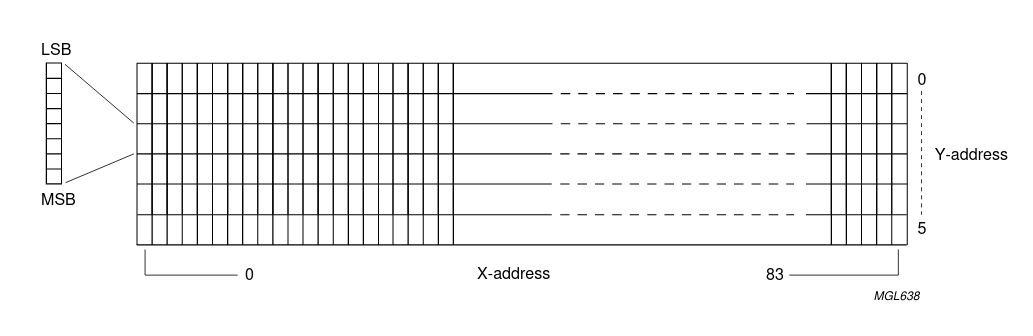
\includegraphics[scale=0.50]{address_display}
    \caption{Adresacja banków pamięci, V=0}
\end{figure}

\paragraph{Inicjalizacja wyświetlacza}
Zaraz po włączeniu zasilania stany rejestrów i pamięci urządzenia są niezdefiniowane.
Należy wygenerować stan niski na linii RST. Następnie na tej samej linii ustawiany
jest stan wysoki.

\begin{center}
\begin{lstlisting}[language=C, basicstyle=\footnotesize]
void displayReset()
{
    LL_GPIO_ResetOutputPin(DISPLAY_PORT, DISPLAY_RST);
    LL_GPIO_SetOutputPin(DISPLAY_PORT, DISPLAY_RST);
} 
\end{lstlisting}
\end{center}

Następnie należy wysłać serię komend:

\begin{enumerate}
    \item Rozszerzony tryb komend
    \item Ustawienie kontrastu
    \item Współczynnik temperatury
    \item Współczynnik biasu
    \item Powrót do regularnego trybu komend
\end{enumerate}


\paragraph{Wysyłanie komend/danych}
Aby wysłać do wyświetlacza komendę należy ustawić na linii DC stan wysoki. Wysyłanie danych
jest oznaczone stanem niskim. Obydwie operacje odbywają się za pomocą interfejsu SPI.
\paragraph{Datasheet}
\url{https://www.sparkfun.com/datasheets/LCD/Monochrome/Nokia5110.pdf}

\subsubsection{Czujnik ruchu}

\paragraph{Opis}
Jako czujnik ruchu został wybrany czujnik typu PIR. Jest to urządzenie pasywne.
Czujniki tego typu wykrywają szybkie zmiany temperatury w swoim otoczeniu. Czujniki
PIR charakteryzują się wysoką ilością sygnałów \emph{false-positive}, dlatego też
urządzenie zastosowane w projekcie ma możliwość regulacji czułości, które pomaga
w znacznym stopniu zniwelować ten problem. Komunikacja z czujnikiem jest prosta - wystawia
on stan wysoki (+3V) na wyjściu w sytuacji, kiedy ruch zostanie wykryty.

\paragraph{Datasheet}
\url{https://www.mpja.com/download/31227sc.pdf}

\subsubsection{Bluetooth}
Wybrane przez nas urządzenie umożliwia komunikację poprzez UART.

\paragraph{Datasheet}
\url{http://www.electronicaestudio.com/docs/istd016A.pdf}

\section{Opis funkcjonalności poszczególnych elementów}

Przycisk
\begin{itemize}
    \item AHB1
    \item GPIOA
    \item NVIC
    \begin{enumerate}
        \item PIN0 - Stan przycisku
    \end{enumerate}
\end{itemize}

Wyświetlacz
\begin{itemize}
    \item AHB1
    \item APB2
    \item SPI1
    \item GPIOA
        \begin{enumerate}
            \item PIN1 - DC
            \item PIN2 - Podświetlenie
            \item PIN4 - CE
            \item PIN5 - CLK
            \item PIN6 - Reset
            \item PIN7 - DIN
        \end{enumerate}
\end{itemize}

Diody LED
\begin{itemize}
    \item AHB1
    \item GPIOE - PIN8-PIN15 - stany diod LED
\end{itemize}

Czujnik ruchu
\begin{itemize}
    \item AHB1
    \item NVIC
    \item GPIOA
        \begin{enumerate}
            \item PIN3 - Odczyt stanu
        \end{enumerate}
\end{itemize}

Bluetooth
\begin{itemize}
    \item AHB1
    \item APB2
    \item NVIC
    \item USART1
    \item GPIOA
        \begin{enumerate}
            \item PIN9 - USART1 Transmitter
            \item PIN10 - USART1 Receiver
        \end{enumerate}
\end{itemize}

\section{Biblioteki zewnętrzne użyte do zrealizowania projektu}

\begin{itemize}
    \item STM32Cube Low Layer Library - biblioteka STM32
    \item Font ASCII dla Nokia 5110 - SparkFun Electronics
\end{itemize}


%----------------------------------------------------------------------------------------
%	BIBLIOGRAPHY
%----------------------------------------------------------------------------------------
%
%\bibliographystyle{apalike}
%
%\bibliography{sample}
%
%
%----------------------------------------------------------------------------------------


\end{document}